\section{Discussion}
\label{sec:discussion}

This section interprets the empirical findings through the lens of design objectives introduced earlier: transparent reward construction, legality-aware action control, and causal simulation fidelity. We focus on what can be inferred from controlled experimental evidence (see Section~\ref{sec:experiments}) and explicitly separate methodological insights from broader deployment claims, aligning with the evaluation rigour advocated by \citet{zhang2020deep}.

\subsection{Reward Decomposition as an Experimental Instrument}
The principal methodological insight of this manuscript is that reward engineering should be treated as controlled experimentation rather than iterative tuning. The 11-component architecture, together with deterministic per-step logging, enables direct attribution of behavioral changes to specific reward terms. In \Exp{01}, performance does not improve monotonically as components are added; instead, quality degrades and recovers across the schedule before peaking at \variant{r7}. This pattern demonstrates interaction effects that are difficult to diagnose under monolithic scalar objectives, which are commonly used in trading RL to optimize raw return or equity delta \citep{meng2019reinforcement,theate2021application}. Unlike these conventional approaches, which obscure component-level attribution and complicate reward shaping analysis \citep{ng1999policy}, our decomposable framework isolates the specific penalties that suppress excessive trading and the signals that improve entry timing.

\subsection{Behavioral Consequences of Action Granularity}
Endpoint metrics in \Cref{tab:action_space} suggest a return--activity trade-off, but the mechanism is clearer when inspecting action usage directly. \Cref{fig:action_dist_agg} reports aggregate action frequencies for the compared interfaces.

\begin{figure}[!tbp]
\centering
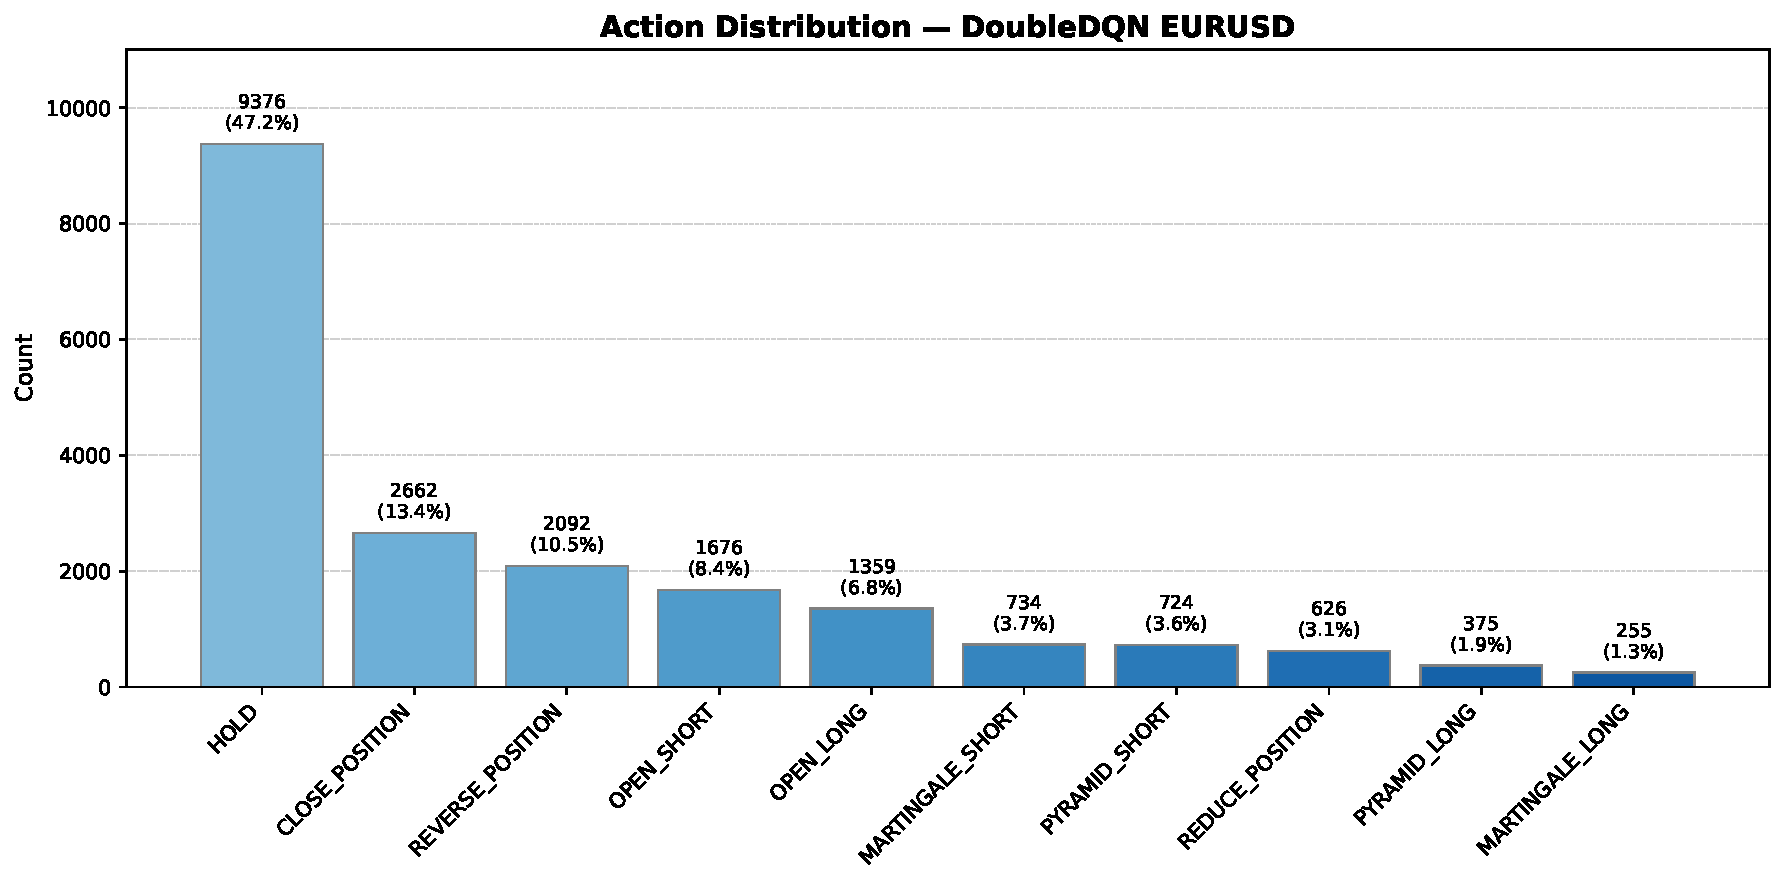
\includegraphics[width=\linewidth]{figures/action_distribution.pdf}
\caption{Aggregate action distributions across training runs, showing broader action usage and higher activity in the extended interface.}
\label{fig:action_dist_agg}
\end{figure}

The distribution shows that richer action semantics are not merely available but actively exploited: scaling, reduction, and reversal primitives contribute substantial policy mass. This explains why the extended interface captures more return opportunities while simultaneously increasing turnover and path volatility.

\subsection{Scaling Mechanics Under Asymmetric Penalties}
The scaling family (\Exp{03}) is best interpreted through both endpoint values (\Cref{tab:scaling}) and operational depth statistics. \Cref{fig:scaling_behavior} visualizes average pyramid and martingale utilization by variant.

\begin{figure}[!tbp]
\centering
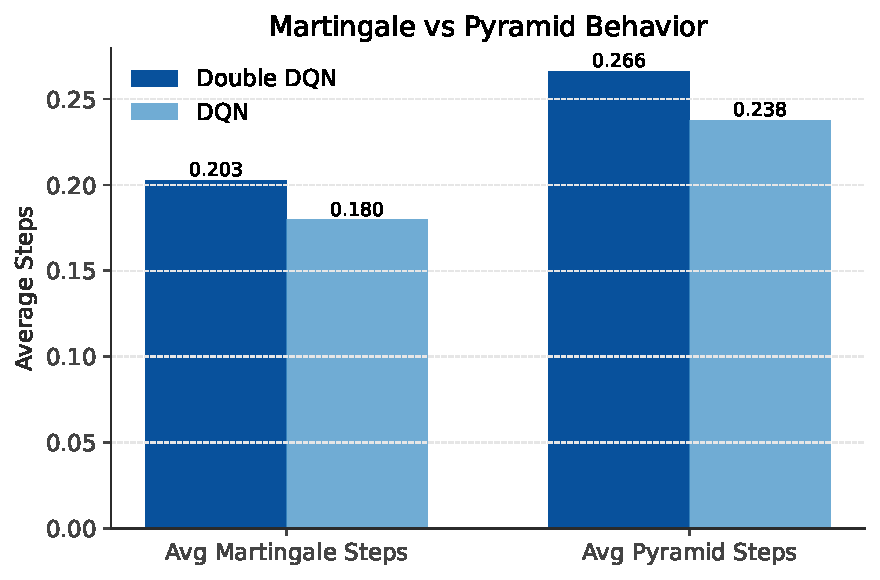
\includegraphics[width=\linewidth]{figures/martingale_pyramid_barplot.pdf}
\caption{Episode-level average pyramid depth (AvgPyr) and martingale depth (AvgMart) by scaling variant.}
\label{fig:scaling_behavior}
\end{figure}

Two implications follow. First, the penalty asymmetry does shape behavior in the intended direction: enabling both mechanisms does not collapse into pure martingale usage. Second, utilization remains bounded, indicating that legality masks and margin controls are actively constraining excessive depth accumulation.

\subsection{Interpreting Endpoint Metrics}
The retained results are intentionally restricted to the experimental scope defined in Section~\ref{sec:experiments}. Under this scope, endpoint metrics are informative about learning behavior but do not establish statistical dominance or deployment readiness. This distinction is central: the manuscript provides evidence about system dynamics, not definitive estimates of out-of-sample expected return. Consequently, directional claims should be interpreted as controlled observations that motivate multi-seed follow-up, in line with reproducibility concerns noted in prior surveys \citep{zhang2020deep}.

\subsection{Layered Safety and Causality Guarantees}
Two cross-cutting properties remain robust across experiments. First, strict anti-lookahead timing is enforced by environment mechanics rather than documentation convention, reducing leakage risk at the API level~\citep{zhang2020deep}. Second, legality masks are applied consistently during both interaction and target computation, following prior invalid-action masking practice~\citep{huang2020closer}. Together with margin and liquidation controls, this yields a defense-in-depth design appropriate for high-risk financial RL experimentation.

\subsection{Practical Interpretation}
For practitioners, the key message is to align architecture choices with deployment objectives: decomposable rewards for auditability, action-space size for desired aggressiveness, and scaling configuration for explicit return--risk preferences, consistent with classical risk-return framing in portfolio analysis~\citep{markowitz1952portfolio}. The present study provides an internally consistent, reproducible baseline for that design process; broader claims require multi-seed and out-of-sample validation.
